\section{Colorizar}

\subsection{Código C}
	El código C se trata de una conjunción de ciclos, el exterior que recorre desde la segunda fila hasta la ante última,  y el interior que recorre desde la segunda columna hasta la última, dejando afuera a todos los bordes, tal como el enunciado pedía. \\ Luego en cada iteración del ciclo interior, que es donde se hacen las opearciones que modifican la imagen, lo que hacemos es crear un arreglo de unsinged chars, "res", que es  donde guardamos los máximos de cada canal en comparación a todos  los pixeles lindantes del píxel en el cual estemos parados (una matriz de 3x3).
\begin{itemize}
\item {Res $[$0$]$ $\leftarrow$ MaximoLindantesAzul}
\item {Res $[$1$]$ $\leftarrow$ MaximoLindantesVerde}
\item {Res $[$2$]$ $\leftarrow$ MaximoLindantesRojo}
\end{itemize}
Luego con estos tres valores calculamos el alpha correspondiente de cada canal por el cual vamos a multiplicar a cada uno. Y por último reescribimos el píxel final, en la imagen src con cada canal multiplicado por dicho alpha.

\subsection{Código ASM}

	El código en ASM se trata también de una unión de ciclos. El ciclo exterior recorre desde la segunda hasta la ante última fila, y el interior recorre las columnas desde la segunda hasta la ante última, pero saltando de a dos píxeles, que es la cantidad que procesamos simultaneamente con instruccciones SSE. \\
	El ciclo interior consta varios pasos, el primero es calcular un registro en el que en las primeras dos DW guardamos los máximos valores de cada canal entre los píxeles lindantes, en sus posiciones respectivas. Se vería asi:\\
\\ACLARACIONES: 
\\ \hspace{3cm} La notacion $X_M{pN}$ es el valor maximo del Color X del el pixel N
\\ \hspace{3cm} Vamos a mostrar solo los primero 8 bytes de los registros Xmm, porque en la parte alta de cada uno hay informacion que vamos a descartar (Fruta).
\par{\textbf{XMM1:}}
\xmmw{$A_M{p2}$}{$R_M{p2}$}{$G_M{p2}$}{$B_M{p2}$}{$A_M{p1}$}{$R_M{p1}$}{$G_M{p1}$}{$B_M{p1}$}
	
 Luego con esta información lo que hacemos es duplicar dicho registro y calcular el máximo de los máximos. Lo que hacemos para lograr esto es shiftear un byte a la derecha al registro duplicado, cosa de poder ir comparando entre ellos a los valores máximos de cada canal, y finalmente reproducimos el valor del máximo entre los máximos en todas las posiciones. El seguimiento de esta operación sería la siguiente: 
\\Vamos a utilizar para esto los registros xmm1, y xmm2

\par{\textbf{XMM2:}}
\xmmw{$A_M{p2}$}{$R_M{p2}$}{$G_M{p2}$}{$B_M{p2}$}{$A_M{p1}$}{$R_M{p1}$}{$G_M{p1}$}{$B_M{p1}$}
\par{\textbf{XMM1:}}
\xmmw{$A_M{p2}$}{$R_M{p2}$}{$G_M{p2}$}{$B_M{p2}$}{$A_M{p1}$}{$R_M{p1}$}{$G_M{p1}$}{$B_M{p1}$}
\par{shifteo un byte a la derecha xmm2 y hacemos pmaxub xmm1,xmm2  máximo entre ambos)}
\par{\textbf{XMM2:}}
\xmmw{$A_M{p2}$}{$R_M{p2}$}{$G_M{p2}$}{$B_M{p2}$}{$A_M{p1}$}{$R_M{p1}$}{$G_M{p1}$}{$B_M{p1}$}

\par{\textbf{XMM1:}}
\xmmw{$Fruta$}{$Fruta$}{$RG_M{p2}$}{$Fruta$}{$Fruta$}{$Fruta$}{$RG_M{p1}$}{$Fruta$}
\par {Notar que ahora mas casillas tienen informacion no relevante al codigo, es información que sera pisada prontamente}
\par{Luego volvemos a shiftear y repetir la operación pmaxub xmm1,xmm2  y queda: }

\par{\textbf{XMM2:}}
\xmmw{$A_M{p2}$}{$R_M{p2}$}{$G_M{p2}$}{$B_M{p2}$}{$A_M{p1}$}{$R_M{p1}$}{$G_M{p1}$}{$B_M{p1}$}

\par{\textbf{XMM1:}}
\xmmw{$Fruta$}{$Fruta$}{$Fruta$}{$RGB_{p2}$}{$Fruta$}{$Fruta$}{$Fruta$}
{{\scriptsize $RGB_{Mp1}$}}
\par{Por último con la instrucción pshuf, dejamos en xmm1 un registro con los máximos de los máximos representado de esta forma: }
\par{\textbf{XMM1:}}
\xmmw{$RGB_{p2}$}{$RGB_{p2}$}{$RGB_{p2}$}{$RGB_{p2}$}{{\scriptsize $RGB_{Mp1}$}}{{\scriptsize $RGB_{Mp1}$}}{{\scriptsize $RGB_{Mp1}$}}{{\scriptsize $RGB_{Mp1}$}}

	 En la segunda parte del código, lo que hacemos es distinguir al maximo entre los maximos. Para esto empezamos haciendo una comparacion entre el registro Xmm1, que tiene en todos sus valores al maximo valor del Pixel 1 y 2 como muestra la imagen anterior, y  el Xmm2 que tiene los maximos parcilaes. De esta manera, quedaria dentro del byte que representaria al color con el valor máximo. una serie de solo "FFFF". Visualmente se puede ver, por ejemplo, sea el caso que el color con el valor maximo del pixel 2 sea el Azul , y el color con el valor maximo del pixel 1, sea el Rojo. El registro Xmm1 se veria de la siguiente forma. 
	 
\par{\textbf{XMM1:}}
\xmmw{$0$}{$0$}{$0$}{$FFFF$}{$0$}{$FFFF$}{$0$}{$0$}

\qquad 	Desde este punto, lo que hacemos, primero es chequear el caso de que algun pixel tenga doble maximo, osea que en dos bytes diferentes se hubiese impreso "FFFF". Y esta solucion es simplemente poner en ceros el byte con el Color de menor prioridad. \\       Ahora  nuestra siguiente operacion, es realizar una funcion auxiliar donde convertimos los valores de este registro Xmm1, si el byte contenia un Cero, ahora va a contener un "-1" ("FFFF" en complemento a 2), y si el Byte contenia "FFFF" ahora va a contener un "1". Y se va a plasmar la informacion sobre el pixel 1 en el registro Xmm0, y la del pixel 2 en Xmm1.\\  Siguiendo el ejemplo anterior los registros qudarian de la siguiente forma:\\  	 ACLARACION: \\ -Ahora los registros ahora van a ser representados completamente pero por sus valores de a doble word. 

\par{\textbf{XMM0:}}
\xmmdw{$-1$}{$1$}{$-1$}{$-1$}

\par{\textbf{XMM1:}}
\xmmdw{$-1$}{$-1$}{$-1$}{$1$}

\par{}
\par{Ahora a estos registros los multiplicamos por el alpha pasado por parametro, y borramos el valor de Color Transparente. Y sumamos uno a todos los colores}
\par{}

\par{\textbf{XMM0:}}
\xmmdw{$1$}{$1+\alpha$}{$1-\alpha$}{$1-\alpha$}

\par{\textbf{XMM1:}}
\xmmdw{$1$}{$1-\alpha$}{$1-\alpha$}{$1+\alpha$}


	Luego como ultimo multiplicamos a cada valor, por el valor respectivo del color que ocupa cada posicion por lo que nos quedan los registros de la siguiente manera:

\par{\textbf{XMM0:}}
\xmmdw{$A_{P1}$}{$R_{P1} * (1+\alpha)$}{$G_{P1}*(1-\alpha)$}{$R_{P1}*(1-\alpha)$}

\par{\textbf{XMM1:}}
\xmmdw{$A_{P2}$}{$R_{P2}*(1-\alpha)$}{$G_{P2}*(1-\alpha)$}{$R_{P2}*(1+\alpha)$}
	
	Lo cuales son los valores ya de los pixeles resultantes. Lo siguiente simplemente es escribirlos correctamente en la imagen resultado, y listo.



	
\subsection{Experimentación 1}

\subsubsection{Idea}
	El primer experimento al igua que en el resto de los filtros, vamos a realizar la comparaciones 
	de cantidad de ciclos, por pixel procesado,  entre los Codigos de C sin optimizar, C optimizado nivel 3, y Asm. En esto vamos a realizar tres comparaciones. La primera trata de comparar entre imagenes cuadradas, como evoluciona el rendimiento con el tamaño de imagen que le pasemos, y Como se ven con respecto a los otros codigos. La segunda comparacion trata de comparar imagenes con la misma cantidad d pixeles, pero con diferentes dimensiones. Y por ultimo comapramos rendimientos al tratar de imagenes con el mismo color en cada pixel.
	
	
\subsubsection{Hipotesis}
	En la primer comparacion esperamos como siempre que el codigo de asm sea el mas optimo, luego le siga el codigo en C optimizado, y por ultimo el codigo de C sin optimizar. \\ 
	En la segunda comparacion, se espera que sea similarla cantidad de ciclos por pixel que se obtiene porque el ciclo no busca ninguna optimizacion respecto al ancho o alto de la imagen, sino que procesa por igual a todos los pixeles.
	Y por ultimo en el tercer experimento suponemos lo mismo, no buscamos ninguna optimizacion con respecto a los valores de los pixeles adyacentes, sino que procesamos por igual a cada pixel indistintamente de su contexto, por lo que esperamos que los valores sean constantes.
	

\subsubsection{Resultados}

\begin{figure}[h!]
\centering
\captionsetup{justification=centering}
	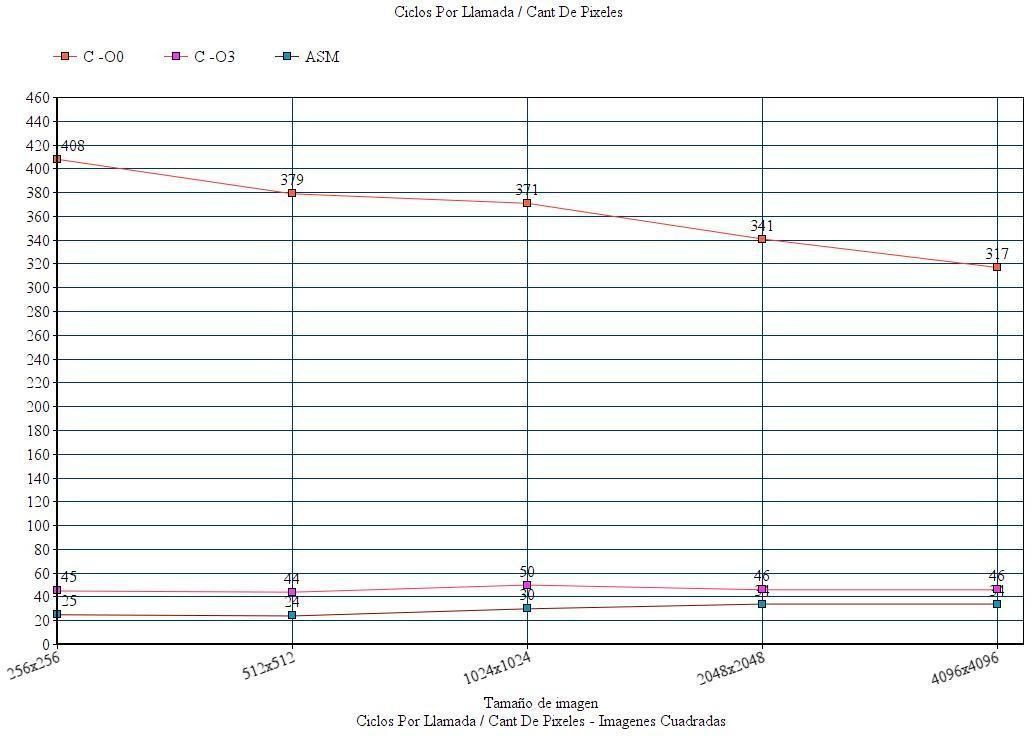
\includegraphics[width = 15 cm, height = 8 cm]{imagenes/ImgCuadradas.jpg}
	\caption[center]{Comparacion diversas implementaciones - Imagenes Cuadradas}
\end{figure}

\medskip
\begin{figure}[h!]
\centering
\captionsetup{justification=centering}
	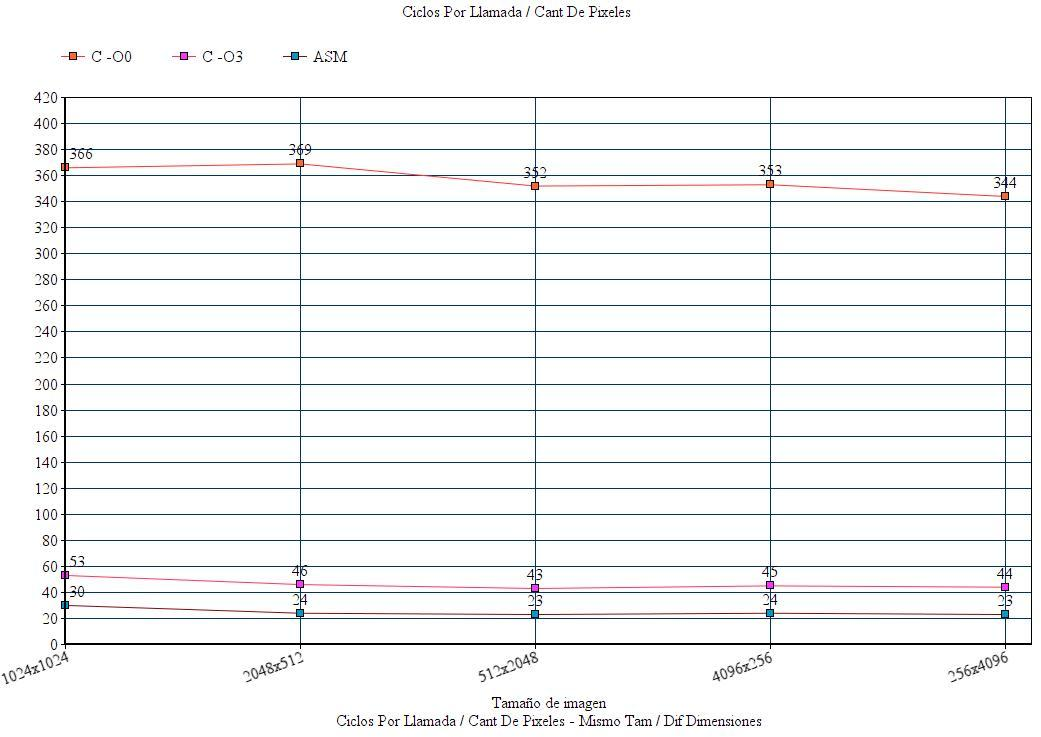
\includegraphics[width = 15 cm, height = 8 cm]{imagenes/DifDimensiones.jpg}
	\caption[center]{Comparacion diversas implementaciones - Diferentes Dimensiones }
\end{figure}

\medskip

\begin{figure}[h!]
\centering
\captionsetup{justification=centering}
	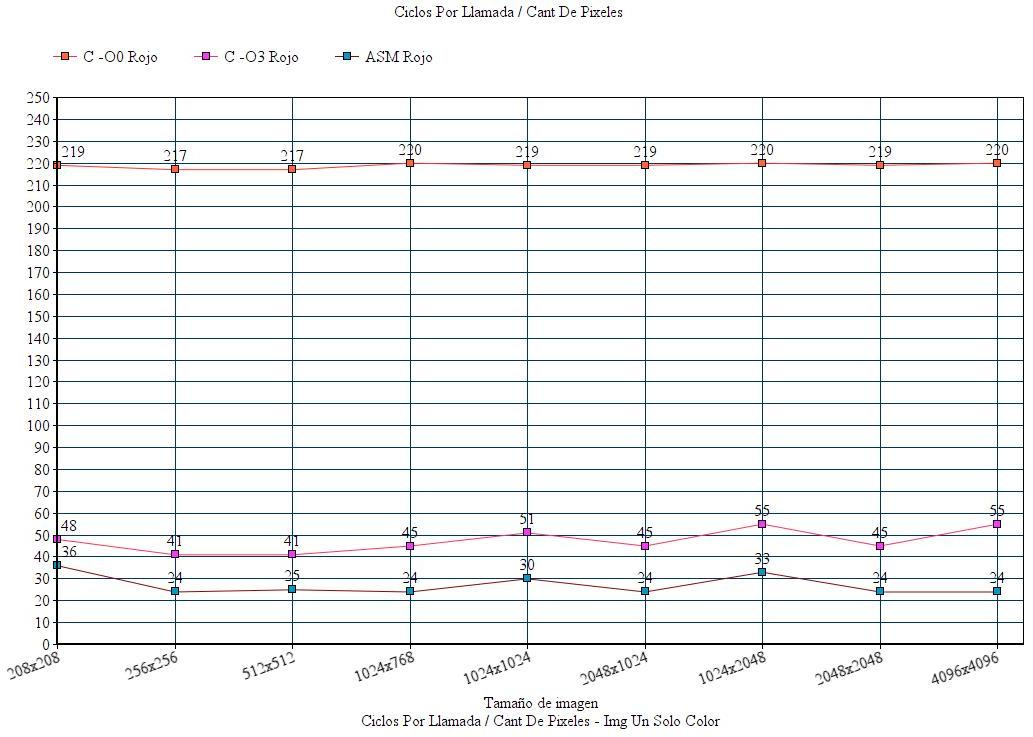
\includegraphics[width = 15 cm, height = 8 cm]{imagenes/mismoColor.jpg}
	\caption[center]{Comparacion diversas implementaciones - Imagenes de un color}
\end{figure}


\subsubsection{Conclucion}
La conclucion que podemos sacar de estas imagenes, es que, en primer lugar, como dijimos en la hipotesis, que se termino corroborando, el codigo en C sin optimizar fue por lejos mas lento que los otros dos. Y el codigo en C optimizado por mas que mejoro muchisimo con respecto al anterior, siguio siendo mas lento que el codigo en asm. \\ Luego podemos ver que no nos confundimos tampoco en el momento de cambiar los tamaño de las imagenes pues los valores se mantuvieron bastantes constantes, y esto porque justamente no se cambia la cantidad de operaciones que se hace respecto a las dimensiones de las imagenes, siempre se mantiene segun la cantidad de pixeles. \\ Por ultimo sin embargo no llamo la atencion el experimento de correr los codigos con imagenes de un solo color. Lo que paso aca de extraño se que bueno los codigos en asm y en C -O3 se mantuvieron cosntantes a los desarrollados con imagenes comunes, sin embargo el codigo en C -O0 demostros una gran mejora respecto a su performance, la cual no podemos explicar bien el porque de ella, y de hecho esto tambien se ve en la primer imagen, donde el las imagenes de 4096x4096 el codigo en C -O0 mostro que mejoraba su rendimiento. Y la explicacion que le asignamos a eso es que justamente porque las imagenes que le pasamos tienen grandes secciones con pixeles del mismo color, porque son eexpanciones de una imagen de 512x512. Y se genera en estos fragmentos esta optimizacion que no podemos explicar sobre C -O0 en imagenes donde el color no cambia.

	

\subsection{Experimentacion 2}	

\subsubsection{Idea}
	El segundo experimento, es un experimento mas destructivo. Vamos a intentar molestar al jump predictor y ver como influye eso en la  performance del programa. 
	El experimento en si trata de agarrar un numero arbitrario desde los datos de entrada y en diferentes puntos de parada, ejecutar un control de flujo if then else, tal que dependiendo de ciertas condiciones random de este numero arbitrario, salte  a diferentes secciones del codigo. TOdo esto dispuesto de tal manera que sea transparente a la ejecucion final del programa, osea si el codigo sigue el camino del if no cambia a si siquue el camino del else.

\subsubsection{Hipotesis}
	Nuestra hipotesis es que justamente el codigo no modificado va a ser bastante mas optimo al codigo desarrollado con molestias para el jump predictor, porque en caso de funcionar estas, en cada ciclo estariamos haciendo que flushee el pipeline, y que pierda muchos ciclos de clock extra.
	
\subsubsection{Resutltados}

\medskip\begin{figure}[h!]
\centering
\captionsetup{justification=centering}
	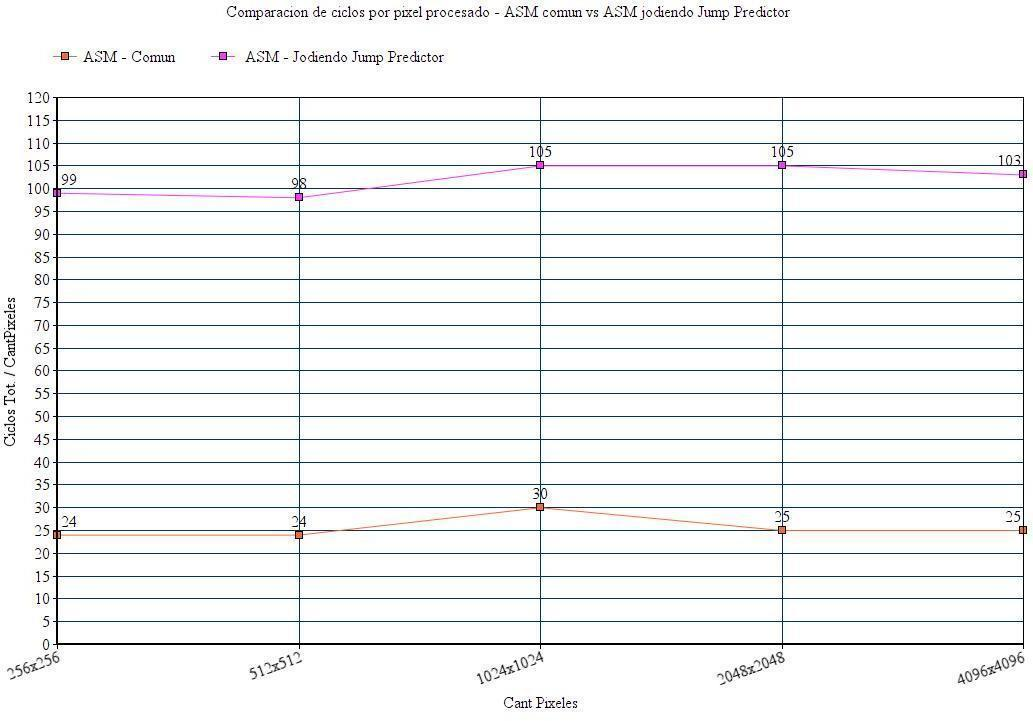
\includegraphics[width = 15 cm, height = 8 cm]{imagenes/JumpPredictor.jpg}
	\caption[center]{Comparacion Asm comun vs Asm molestando Jump Predictor}
\end{figure}

\medskip

\subsubsection{Conclucion}
Efectivamente los resultados fueron los esperados, por lo que nos llevamos como conclucion del experimento que influye mucho la arbitrareidad del flujo del programa que armes, si uno lo hace muy random como en este caso, por mas que no afecte a la complegidad total el programa tarda significativamente mas.

\subsection{Experimento 3}

\subsubsection{Idea}
En el tercer experimento vamos a ver hasta que punto es optimo aplicar la tecnica de unrolling sobre un codigo. Osea lo que planeamos hacer es correr el codigo de colorizar, sobre una imagen de 1024x1024, desenrrollando el ciclo interior, distinta cantidad de veces, vamos a empezar desenrrollando 16, luego 32, y luego completamente.

	   
\subsubsection{Hipotesis}
Lo que esperamos de este experimento es que el codigo desenrrollado 16 y 32 veces, mantenga el nivel de performance con el que demuestra normalmente, o un poco mas optimo, y esto porque en s\'i el codigo de colorizar lleva muchas instrucciones, por lo que los pasos que nos ahorramos al desenrrollar el codigo no es significativo en el total del programa. Sin embargo en el caso de desenrrollar todo el codigo, esperamos una mucha peor performance por parte del codigo y esto debido a que el tamaño del codigo aumentaria enrmomente su tamaño de modo que no entre en la memoria cache el mismo, y deba empezar a hacer lecturas de memoria para leer las instrucciones.
	
\subsubsection{Resultados}

\begin{figure}[h!]
\centering
\captionsetup{justification=centering}
	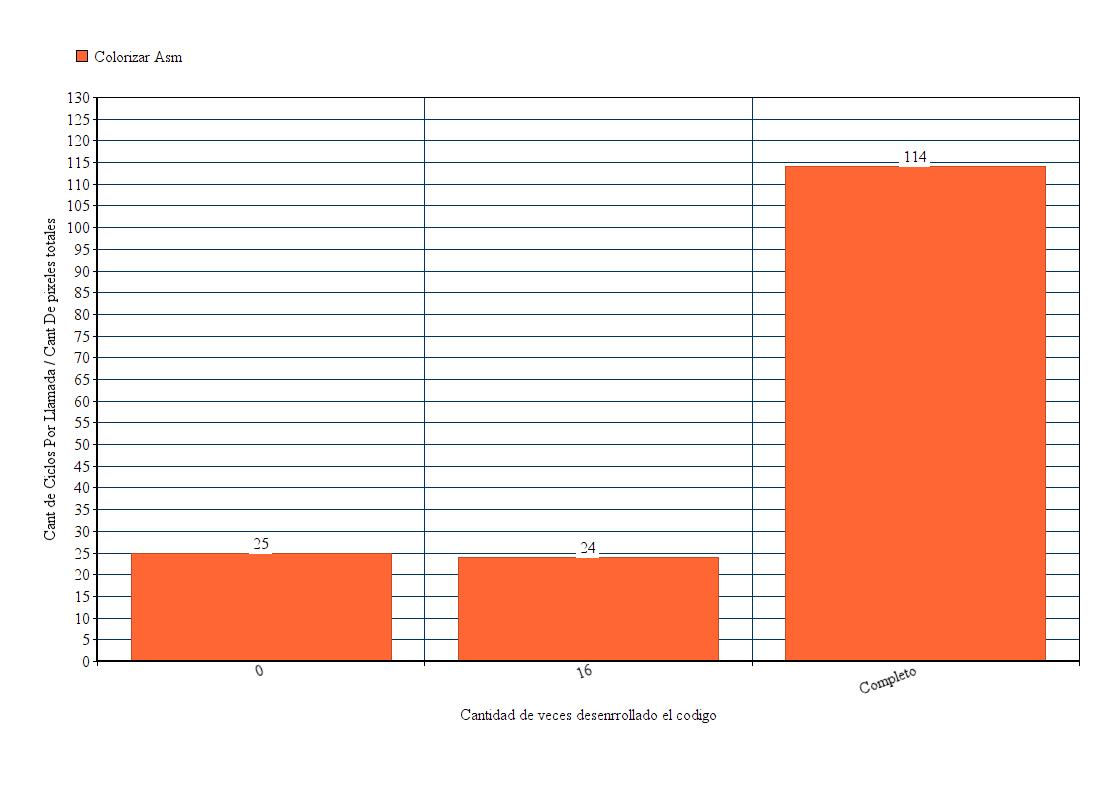
\includegraphics[width = 15 cm, height = 8 cm]{imagenes/unroll.jpg}
	\caption[center]{Comparacion Asm común vs Asm unrrolling 16  vs Asm Unrrolling Completo}
\end{figure}

\medskip

	
\subsubsection{Conclusión}
La conclucion que sacamos de este esxprimento es que la tecnica de desenrrollar codigo es efectiva para pequeños whiles, porq eliminas algunas instrucciones inecesarias, sin embargo ya para un while de un tamaño mayor a lo usual, la optimizacion generada por esto se diluye hasta el punto d  no notarse. Ademas de que efectivamente elementos como la memoria cache son limitantes aca, donde pasa que los problemas de lectura a memoria dejan de ser parte de como esta hecho el algoritmo y pasa a ser a simplemente poder leerlo. 
 
